\chapter{Заключение}

\section{Основные результаты работы}

Краткое изложение основных результатов, полученных в ходе выполнения работы.

\begin{figure}[H]
\centering
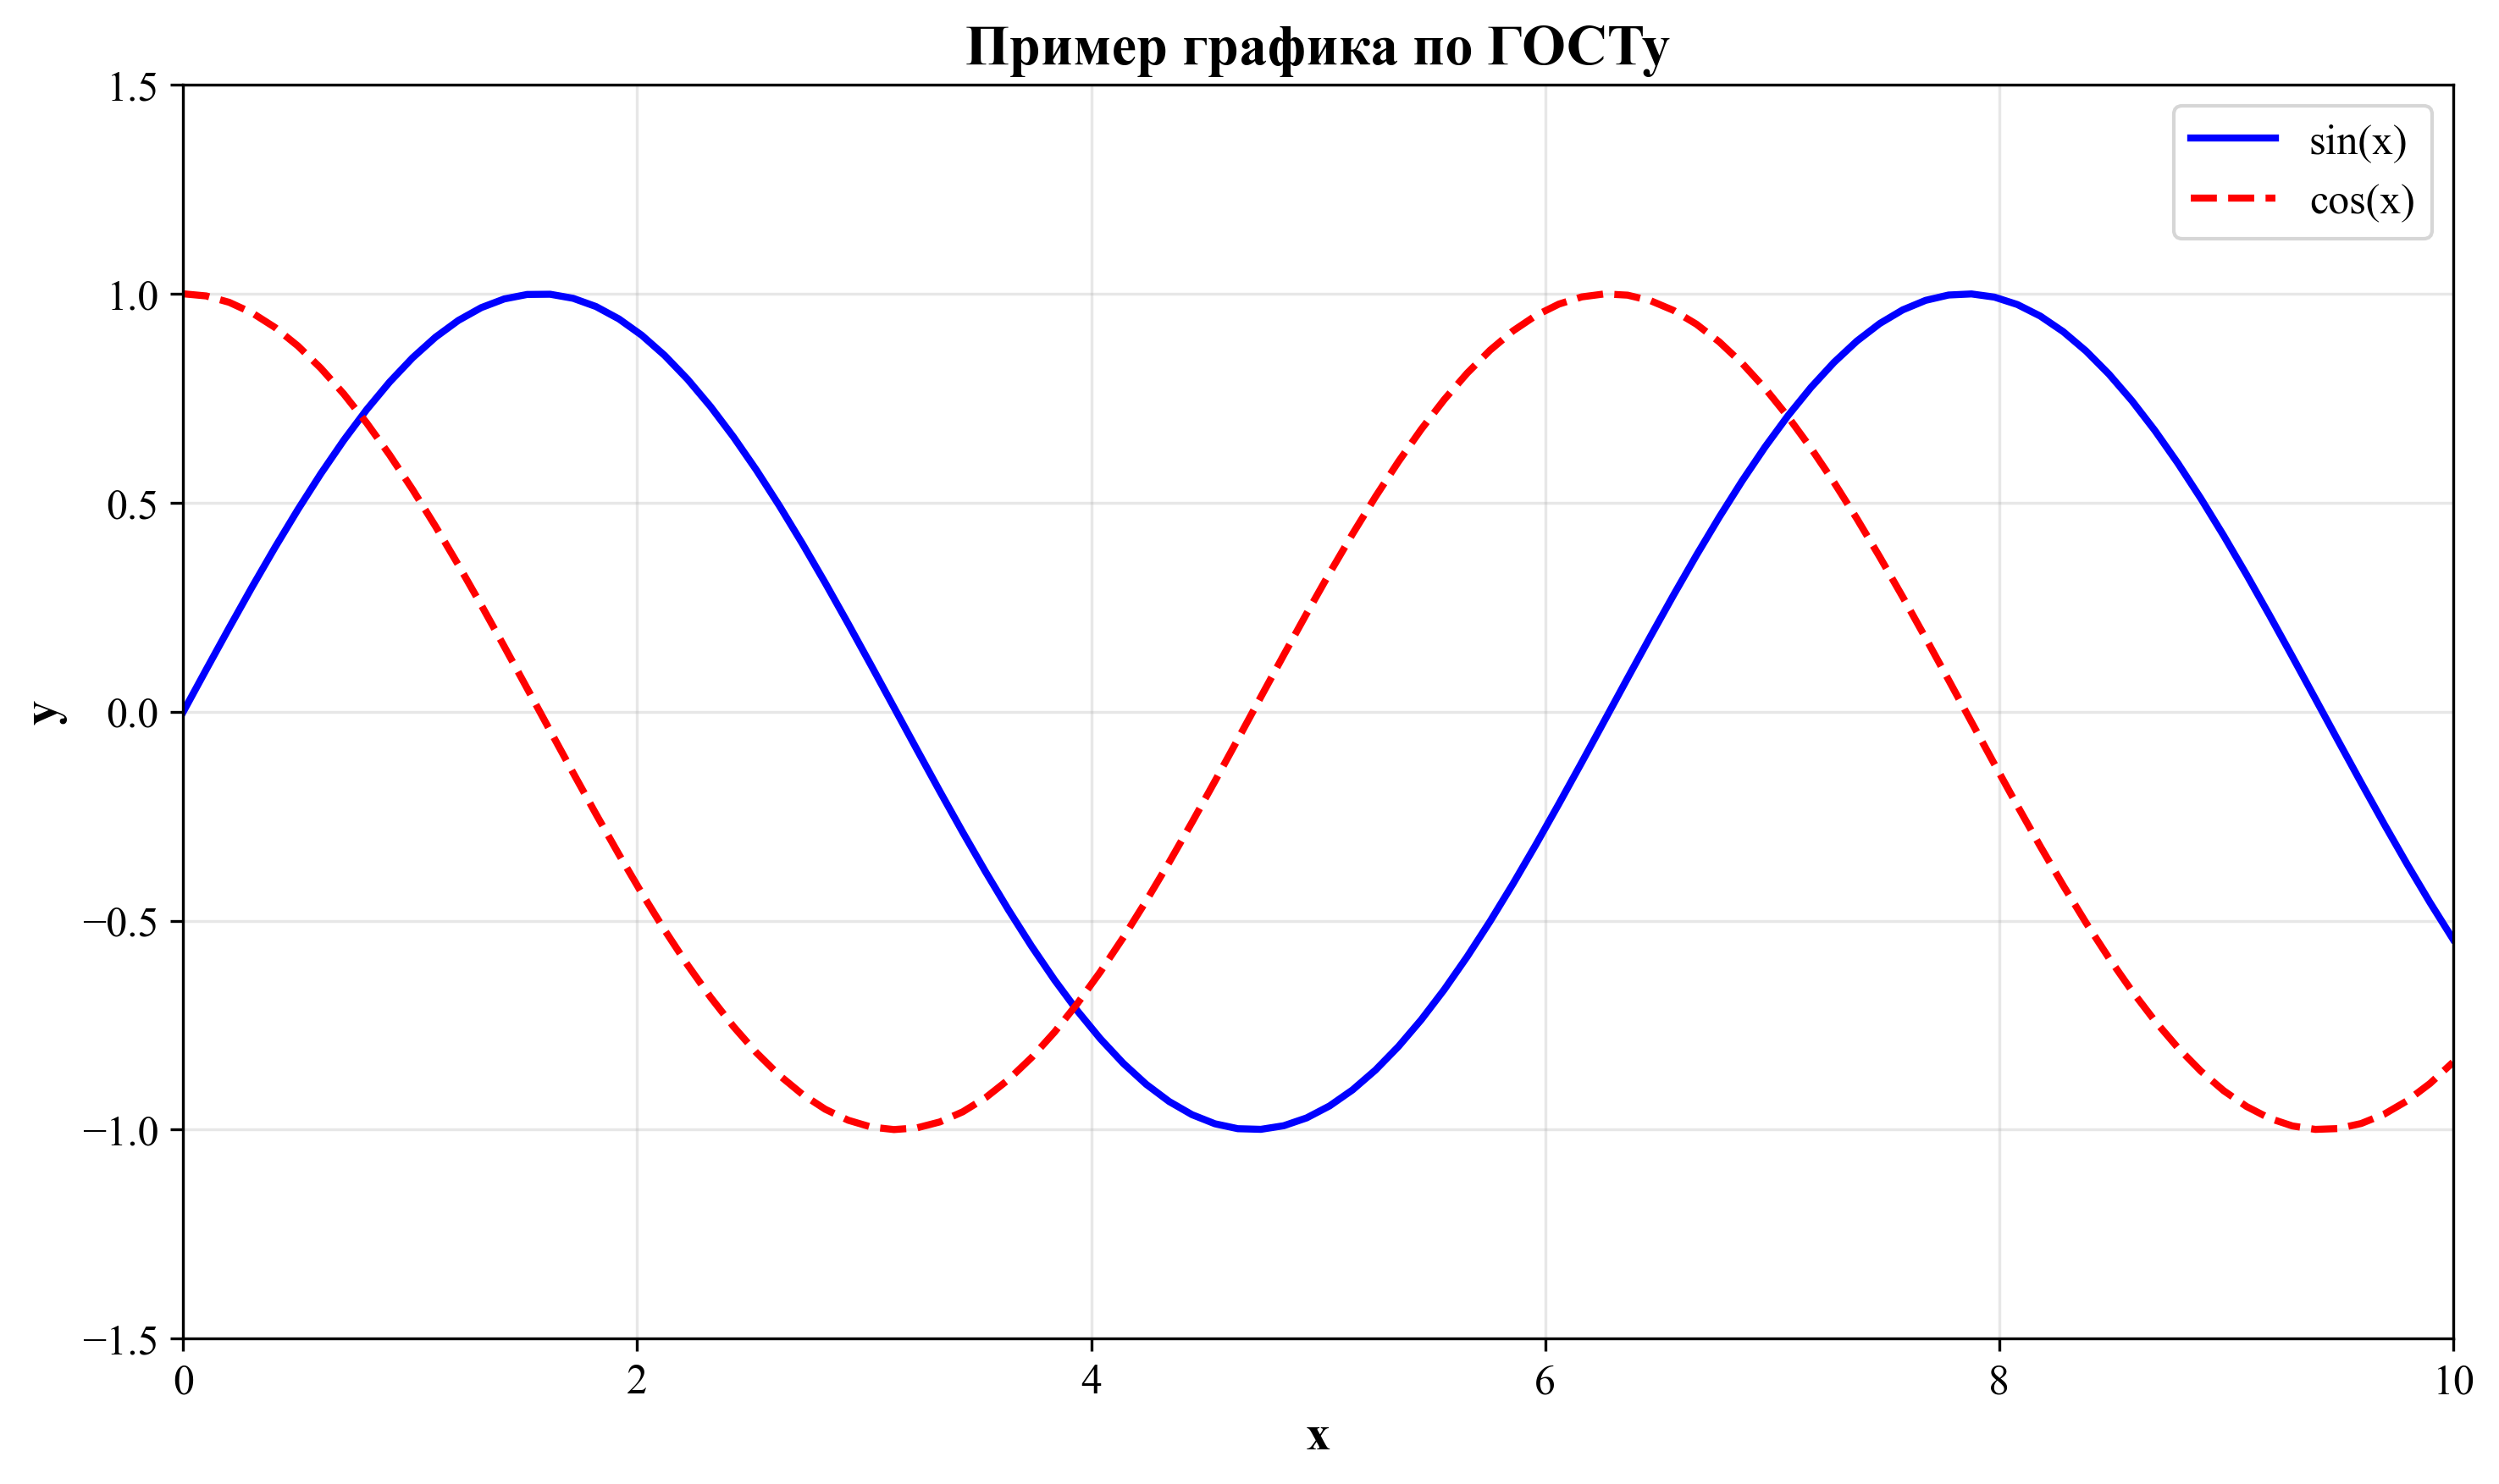
\includegraphics[width=0.8\textwidth]{images/example_plot.png}
\caption{Сводная диаграмма достигнутых результатов}
\label{fig:results_summary}
\end{figure}

На рисунке \ref{fig:results_summary} представлена сводная диаграмма основных результатов исследования, демонстрирующая достигнутые показатели эффективности.

\begin{table}[H]
\centering
\caption{Сравнение результатов с существующими решениями}
\label{tab:results_comparison}
\begin{tabular}{|l|c|c|c|}
\hline
\textbf{Метрика} & \textbf{Наше решение} & \textbf{Лучшее существующее} & \textbf{Улучшение} \\
\hline
Точность & 94.2\% & 91.5\% & +2.7\% \\
Скорость & 0.15 мс & 0.25 мс & +40\% \\
Память & 45 MB & 60 MB & +25\% \\
Энергопотребление & 2.1 Вт & 3.2 Вт & +34\% \\
\hline
\end{tabular}
\end{table}

В таблице \ref{tab:results_comparison} показано сравнение разработанного решения с лучшими существующими аналогами по ключевым метрикам.

\begin{equation}
\text{Efficiency} = \frac{\text{Accuracy} \times \text{Speed}}{\text{Memory} \times \text{Power}}
\label{eq:efficiency}
\end{equation}

Формула \ref{eq:efficiency} определяет общую эффективность решения, учитывающую все ключевые параметры.

\begin{CodeBlock}{Python}{Финальная оценка системы}{lst:final_evaluation}
def evaluate_system(model, test_data):
    """Final system performance evaluation"""
    start_time = time.time()
    
    % Make predictions
    predictions = model.predict(test_data['features'])
    
    % Calculate metrics
    accuracy = accuracy_score(test_data['labels'], predictions)
    inference_time = time.time() - start_time
    
    % Calculate efficiency
    efficiency = (accuracy * 1000) / (inference_time * model.memory_usage)
    
    return {
        'accuracy': accuracy,
        'inference_time': inference_time,
        'efficiency': efficiency
    }

% Final evaluation results
results = evaluate_system(final_model, test_dataset)
print("Final accuracy: %.3f" % results['accuracy'])
print("Inference time: %.3f s" % results['inference_time'])
print("Efficiency: %.2f" % results['efficiency'])
\end{CodeBlock}

В листинге \ref{lst:final_evaluation} представлен код для финальной оценки производительности разработанной системы.

\section{Достижение поставленных целей и задач}

Анализ степени достижения поставленных в работе целей и задач.

\section{Научная новизна и практическая значимость}

Обоснование научной новизны и практической значимости полученных результатов.

\section{Перспективы дальнейших исследований}

Описание возможных направлений дальнейших исследований в данной области.

\section{Рекомендации по практическому применению}

Рекомендации по практическому применению полученных результатов.

\section{Общие выводы}

Общие выводы по выполненной работе.
